
\section{Resultados dos testes e sua discussão}


Dada a complexidade e as dificuldades associadas ao teste de
protocolos distribuídos para controlo de equipamentos de rede num
contexto real, é comum recorrer a emulação para teste dos mesmos. Os
primeiros emuladores recorriam a máquinas reais, interligadas através
de um sistema de emulação do tempo de trânsito e da perda de pacotes
numa rede real [ModelNet].

Tal como discutido em \ref{introducao}

Foram então realizados múltiplos testes que estudavam a variação das variáveis descritas em \ref{benchs}, nomeadamente a variação do débito e a variação do número de instâncias. Foi também ainda realizado um teste de \textit{baseline}, com o objectivo de verificar o peso introduzido pelas comunicações do \textit{mysql} na rede. Serão então apresentados frente a frente os resultados no ambiente de containers \textit{versus} o ambiente de máquinas virtuais.


\begin{center}

	\begin{figure}[H]
		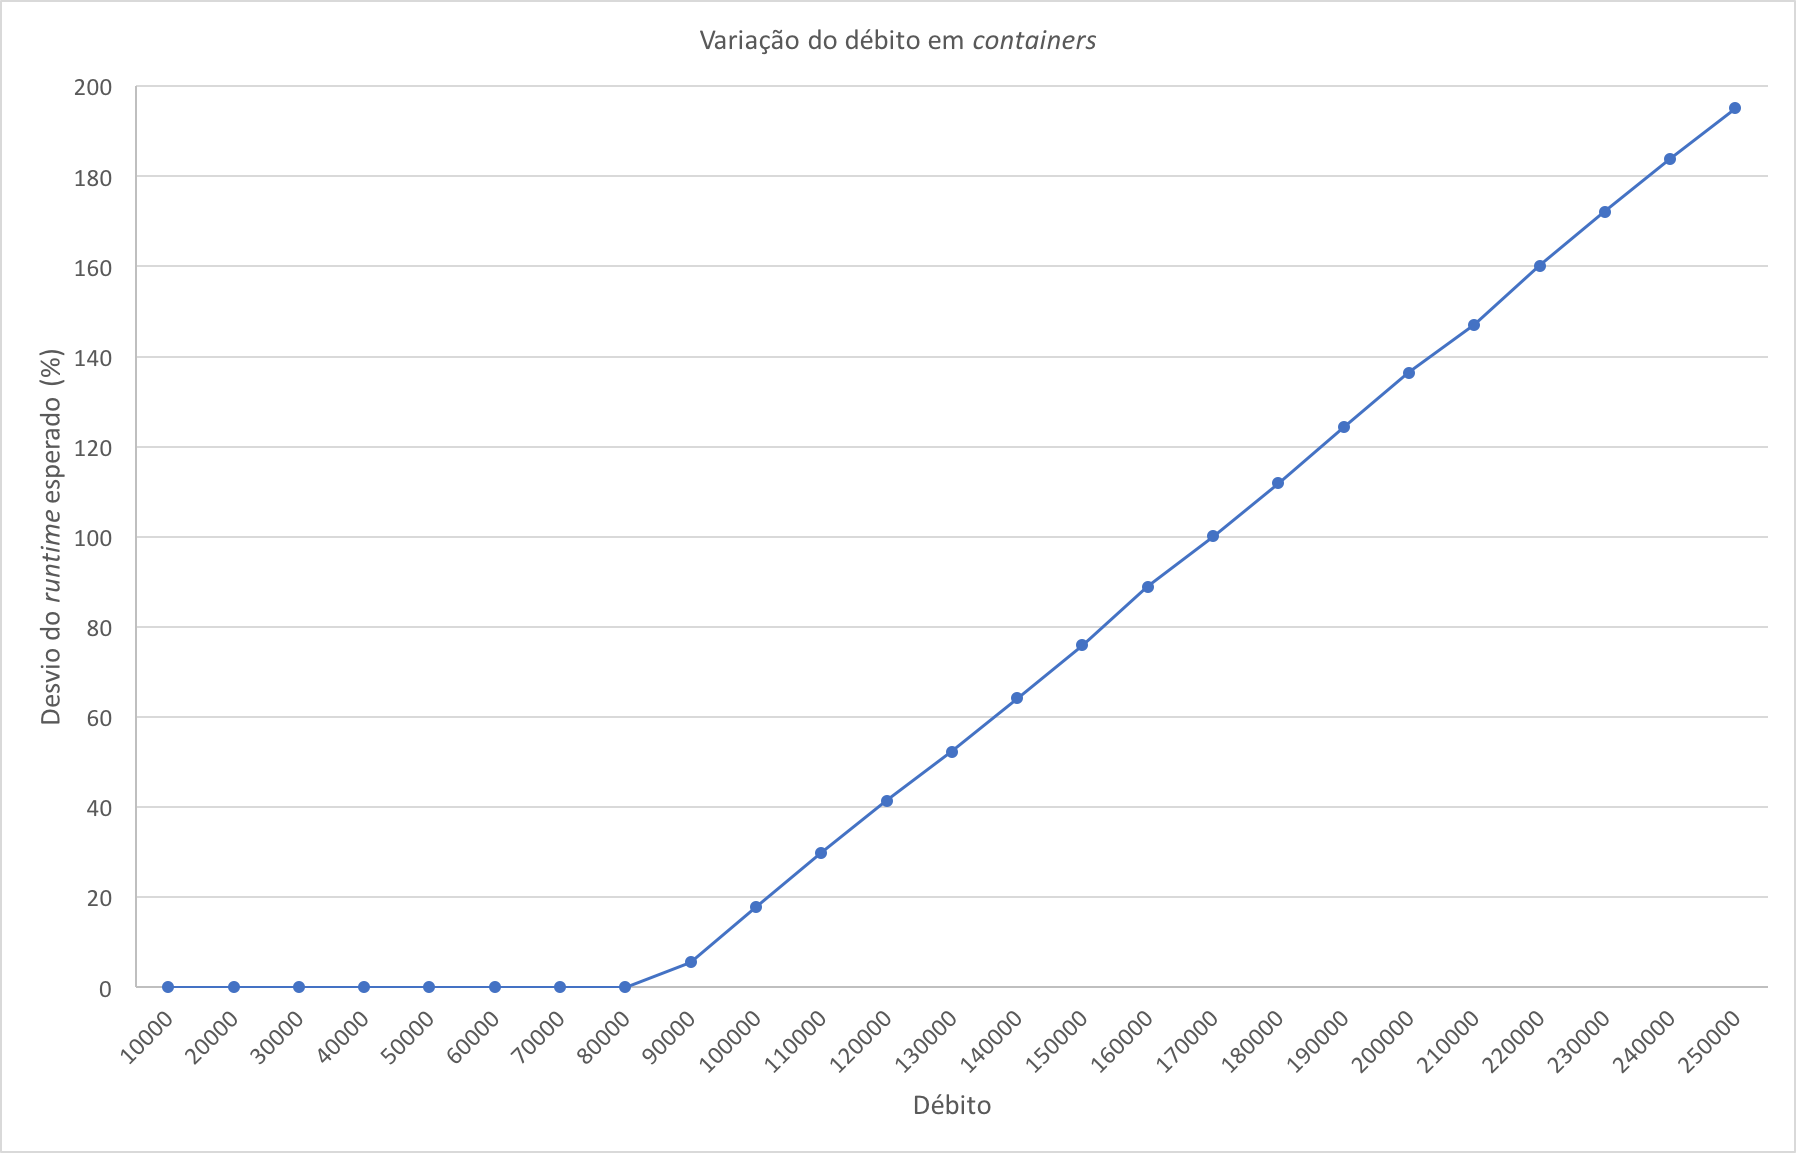
\includegraphics[scale=0.4]{figures/Containers/docker-ins.png}
		\caption{Containers - Variação de inserções por minuto}
		\label{fig:docker-ins}
	\end{figure}

		\begin{figure}[H]
			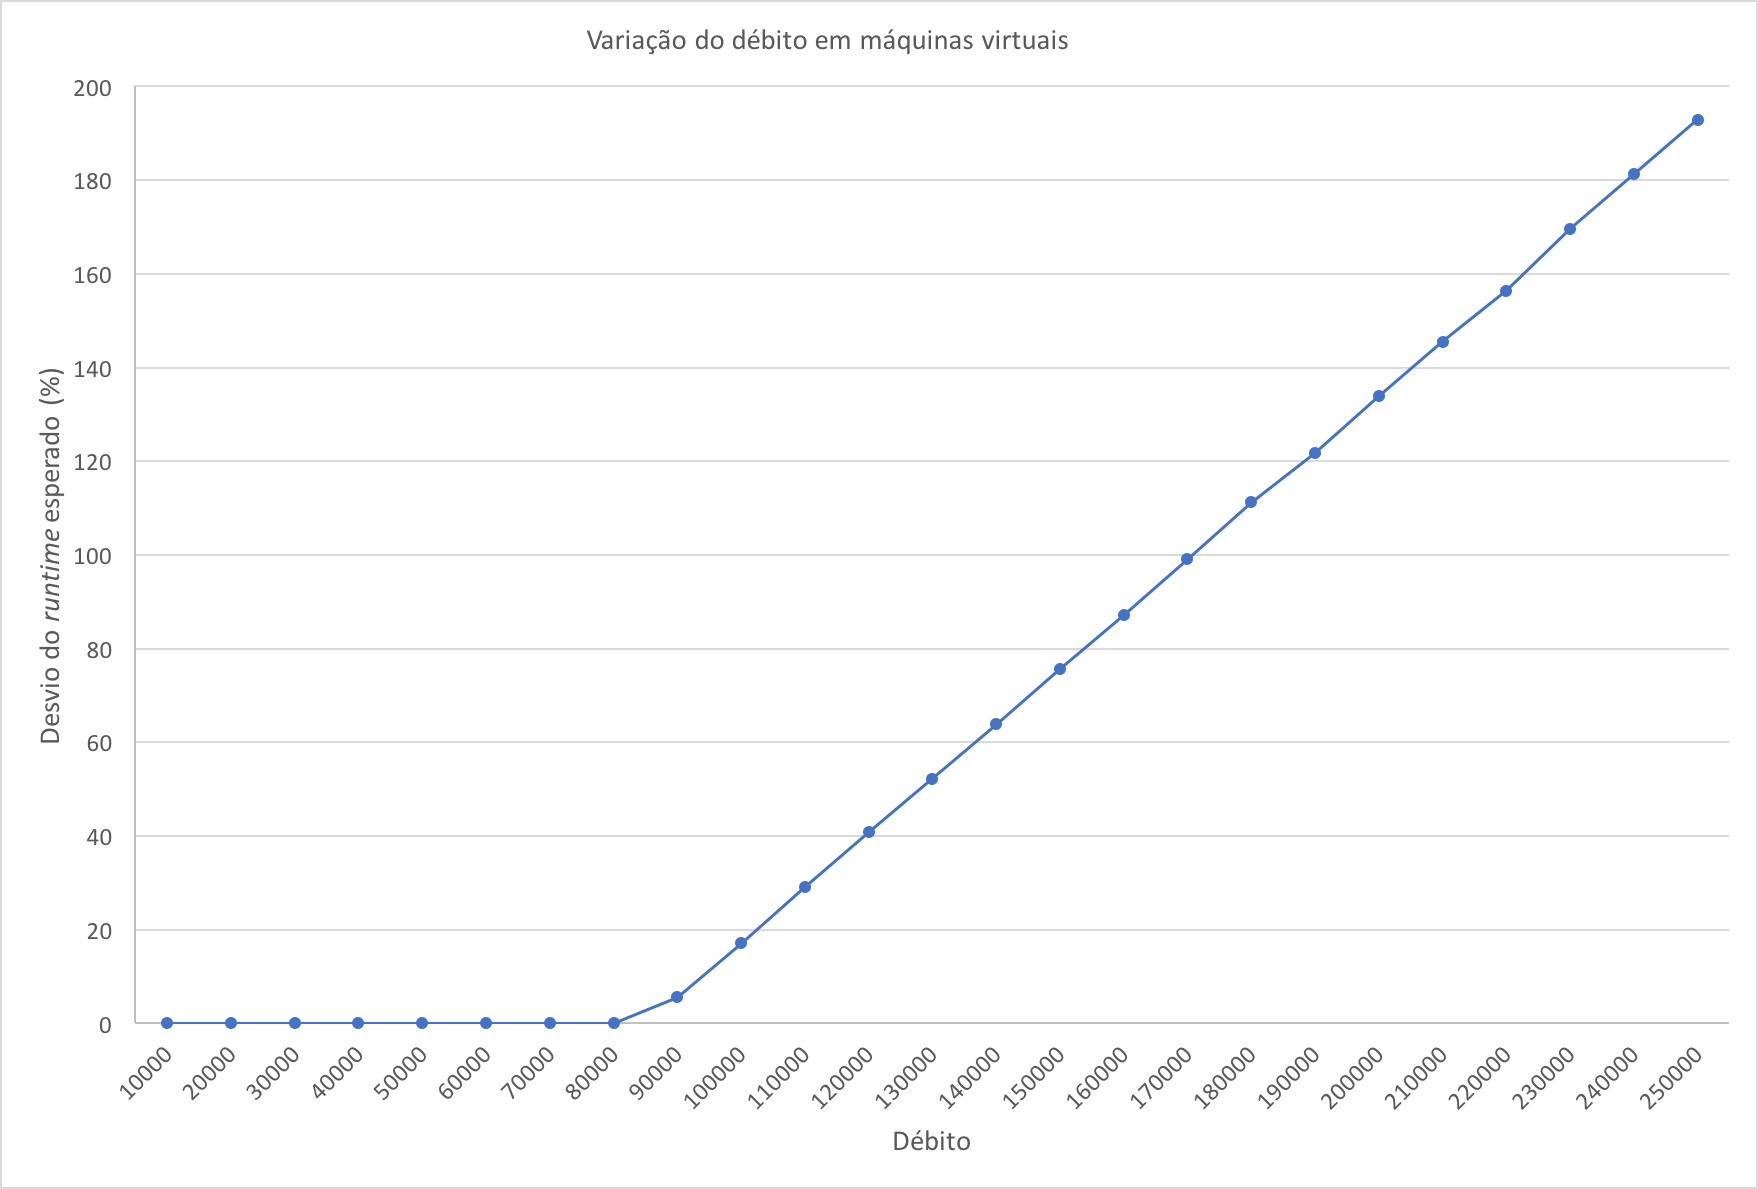
\includegraphics[scale=0.4]{figures/VMs/vms-ins.png}
			\caption{Máquinas Virtuais - Variação de inserções por minuto}
			\label{fig:vms-ins}
		\end{figure}



		\begin{figure}[H]
			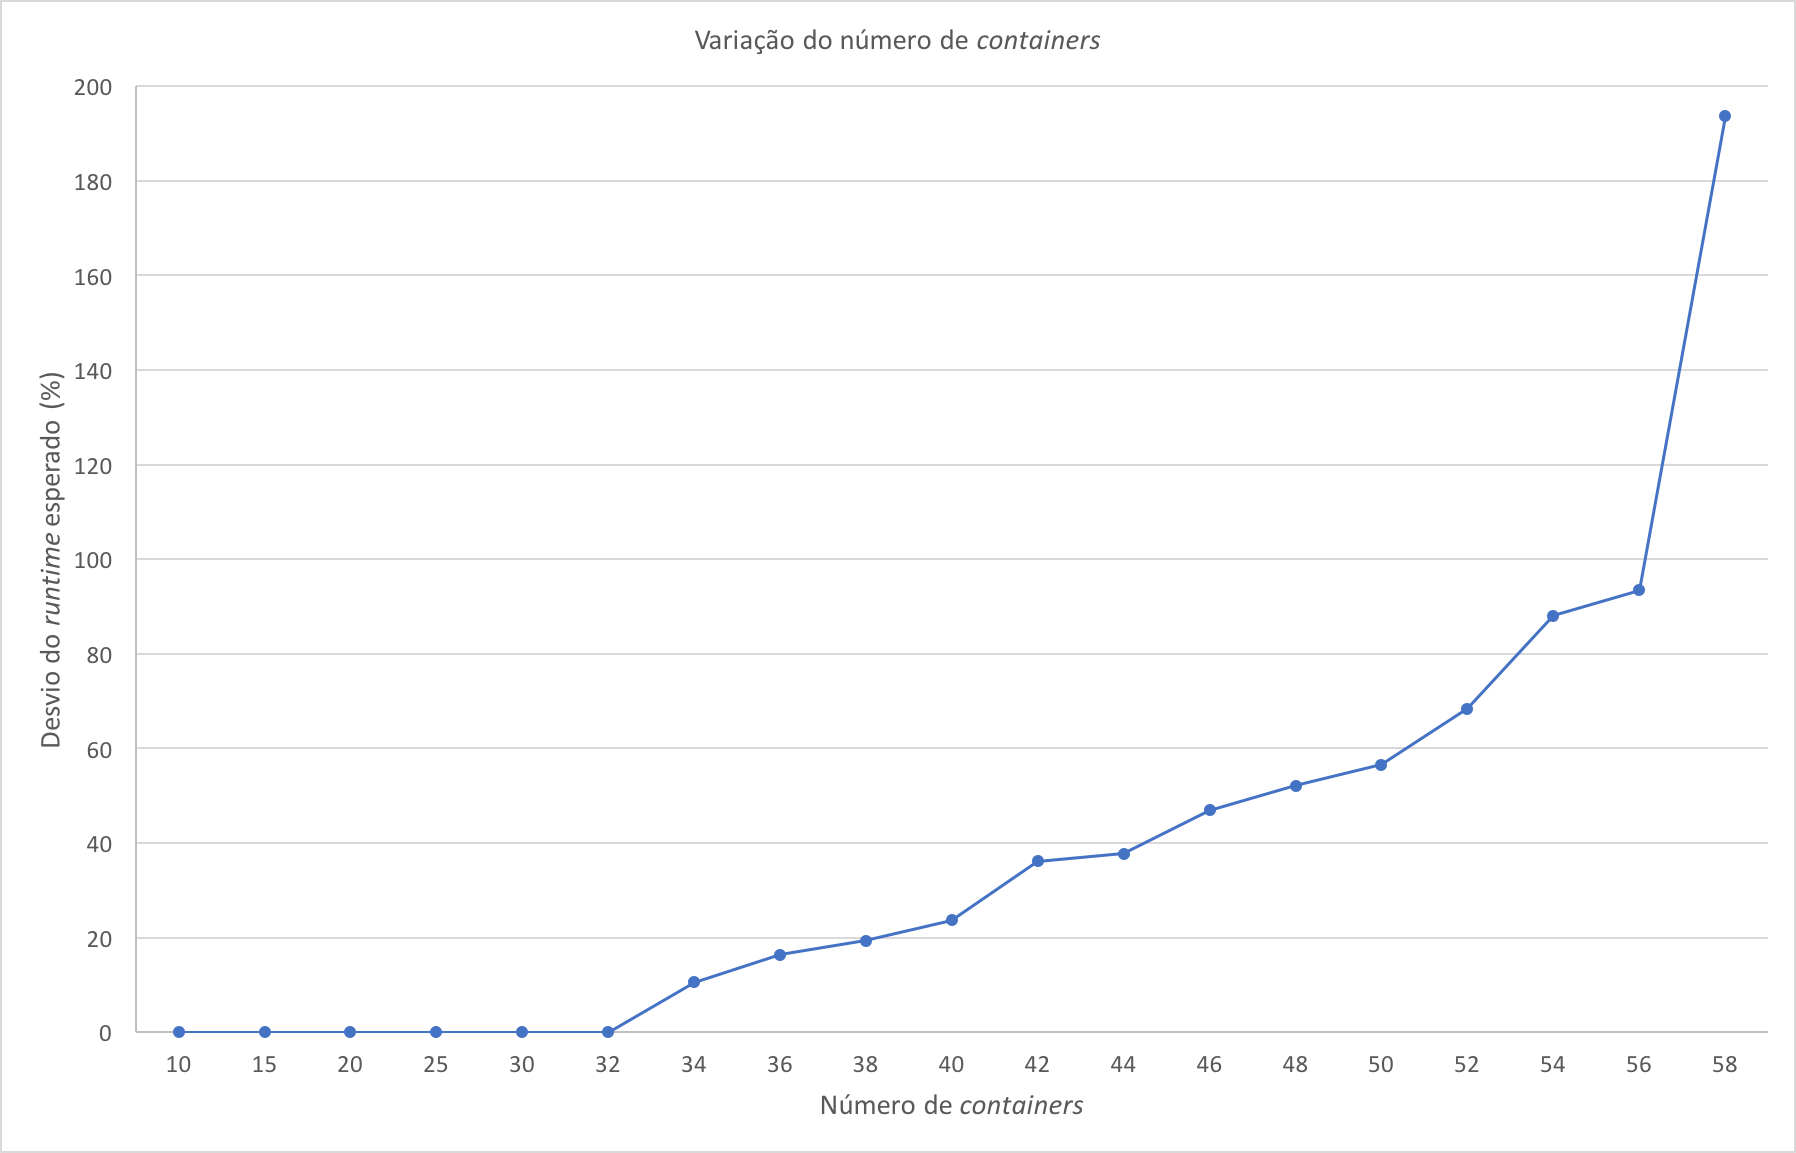
\includegraphics[scale=0.4]{figures/Containers/docker-nos.png}
			\caption{Containers - Variação de instâncias}
			\label{fig:docker-nos}
		\end{figure}

		\begin{figure}[H]
			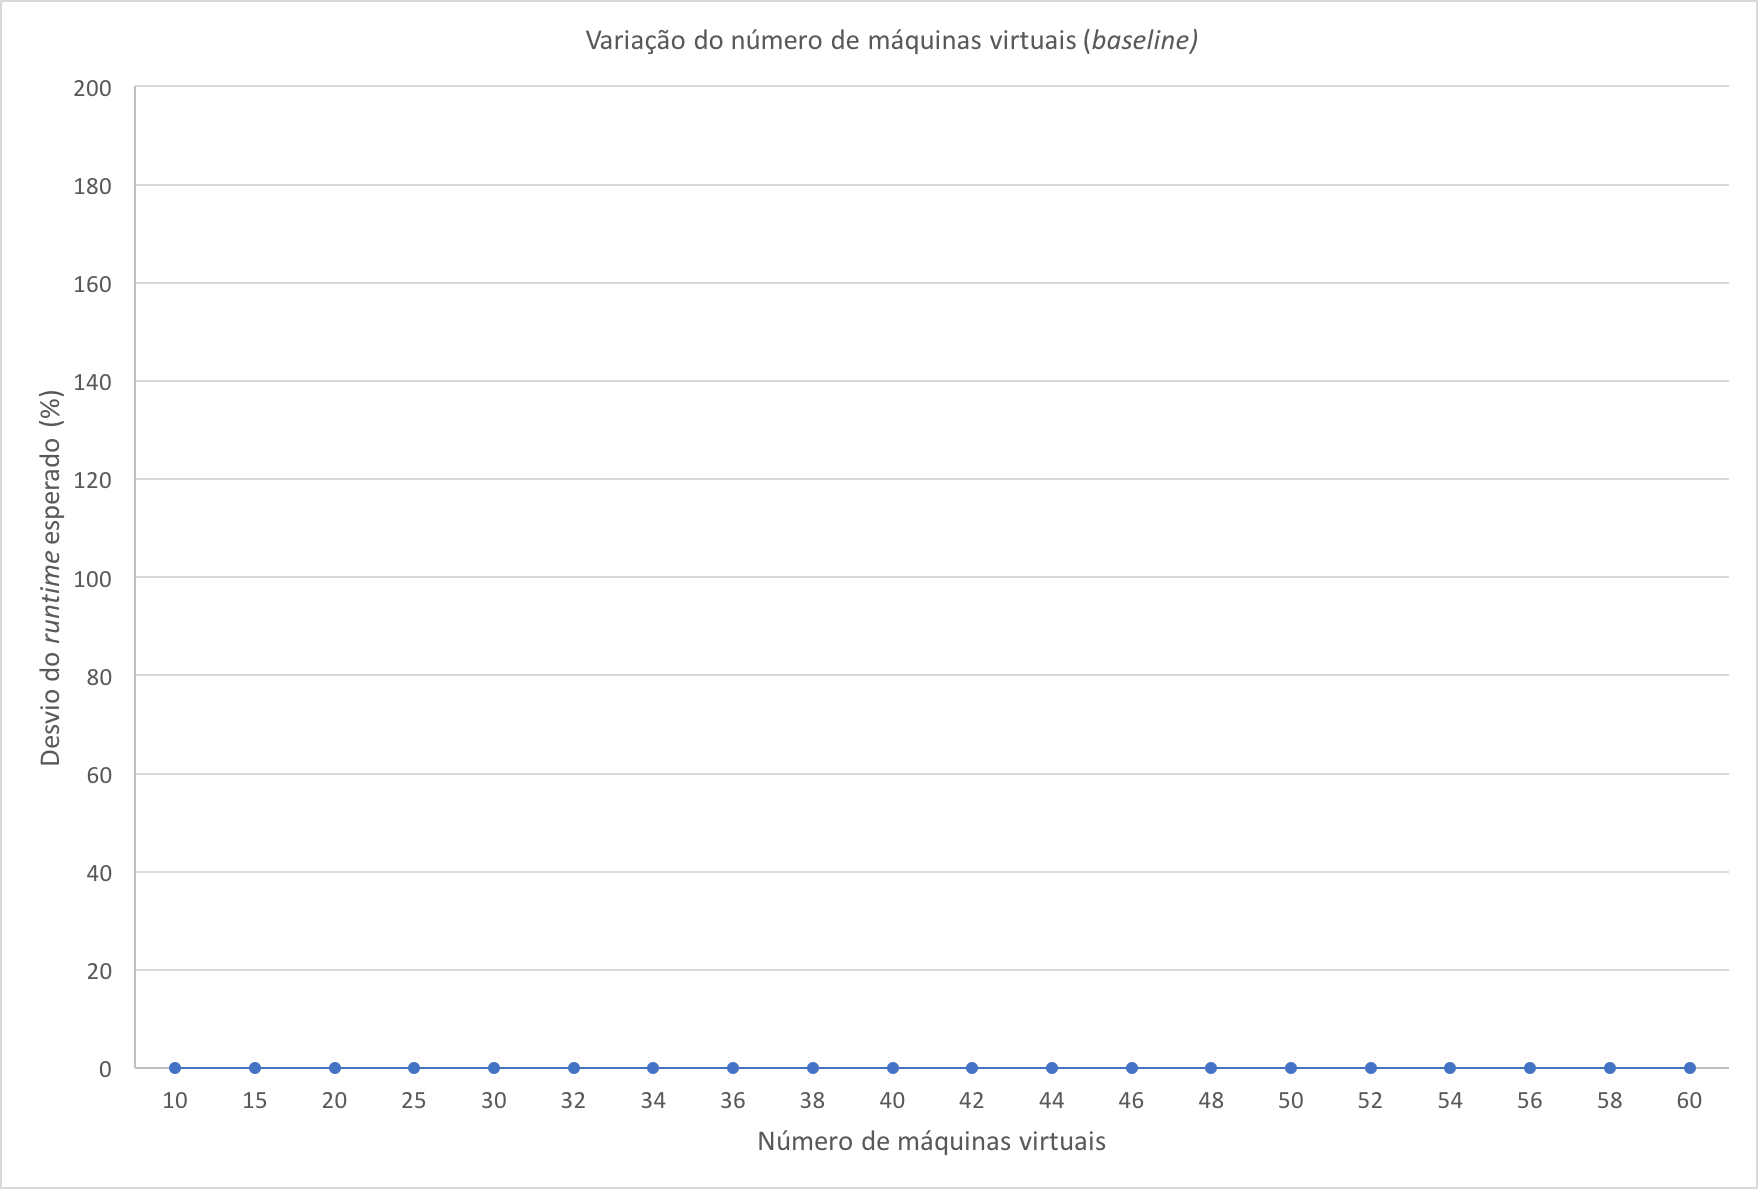
\includegraphics[scale=0.4]{figures/VMs/vms-nos.png}
			\caption{Máquinas Virtuais - Variação de instâncias}
			\label{fig:vms-nos}
		\end{figure}

		\discutir{faltam imagens e comentar}

		\begin{comment}

		\begin{figure}[H]
			\includegraphics[scale=0.4]{figures/Containers/docker-ins-base.png}
			\caption{Containers - Variação de inserções por minuto em modo \textit{baseline}}
			\label{fig:docker-ins-base}
		\end{figure}

		\end{comment}

		\begin{figure}[H]
			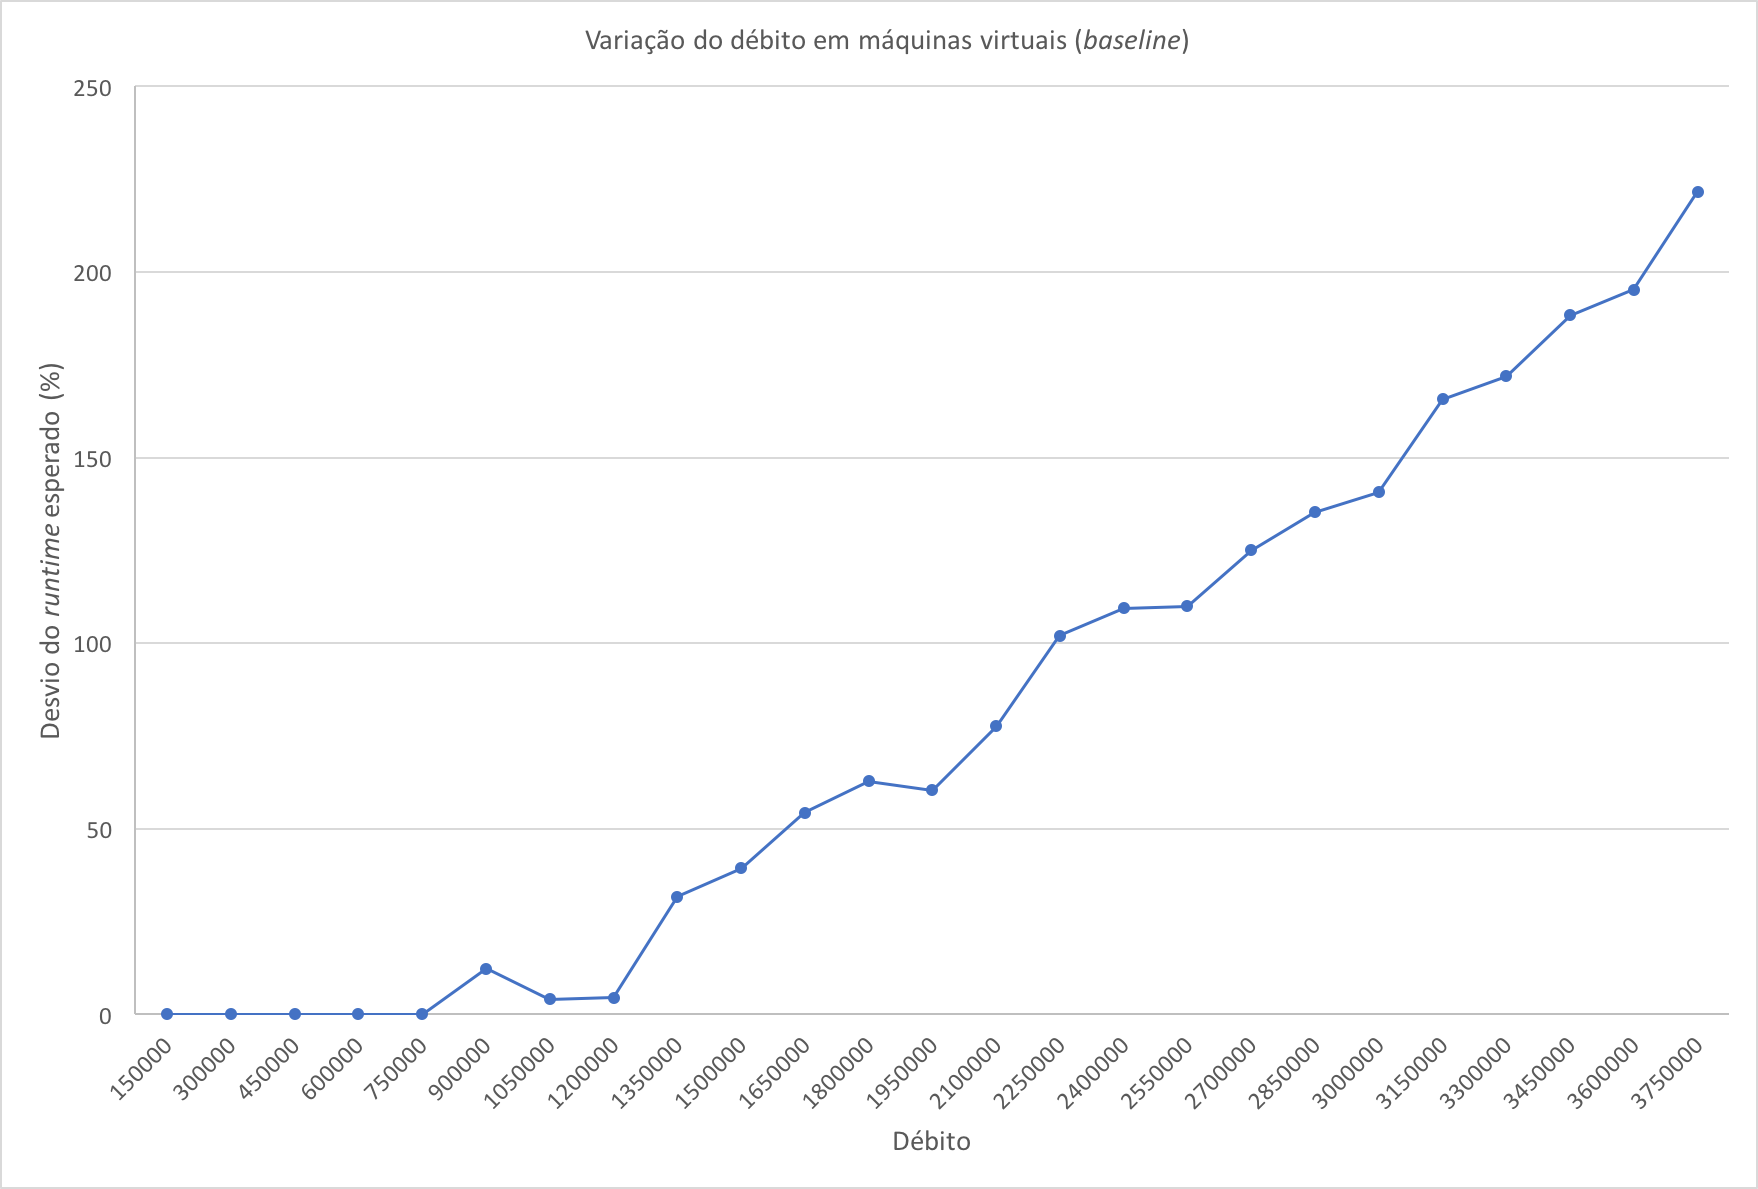
\includegraphics[scale=0.4]{figures/VMs/vms-ins-base.png}
			\caption{Máquinas Virtuais - Variação de inserções por minuto em modo \textit{baseline}}
			\label{fig:vms-ins-base}
		\end{figure}


		\discutir{faltam imagens e comentar}

		\begin{comment}

		\begin{figure}[H]
			\includegraphics[scale=0.4]{figures/Containers/docker-nos-base.png}
			\caption{Containers - Variação de inserções por minuto em modo \textit{baseline}}
			\label{fig:docker-ins-base}
		\end{figure}
		
		\end{comment}

		\begin{figure}[H]
			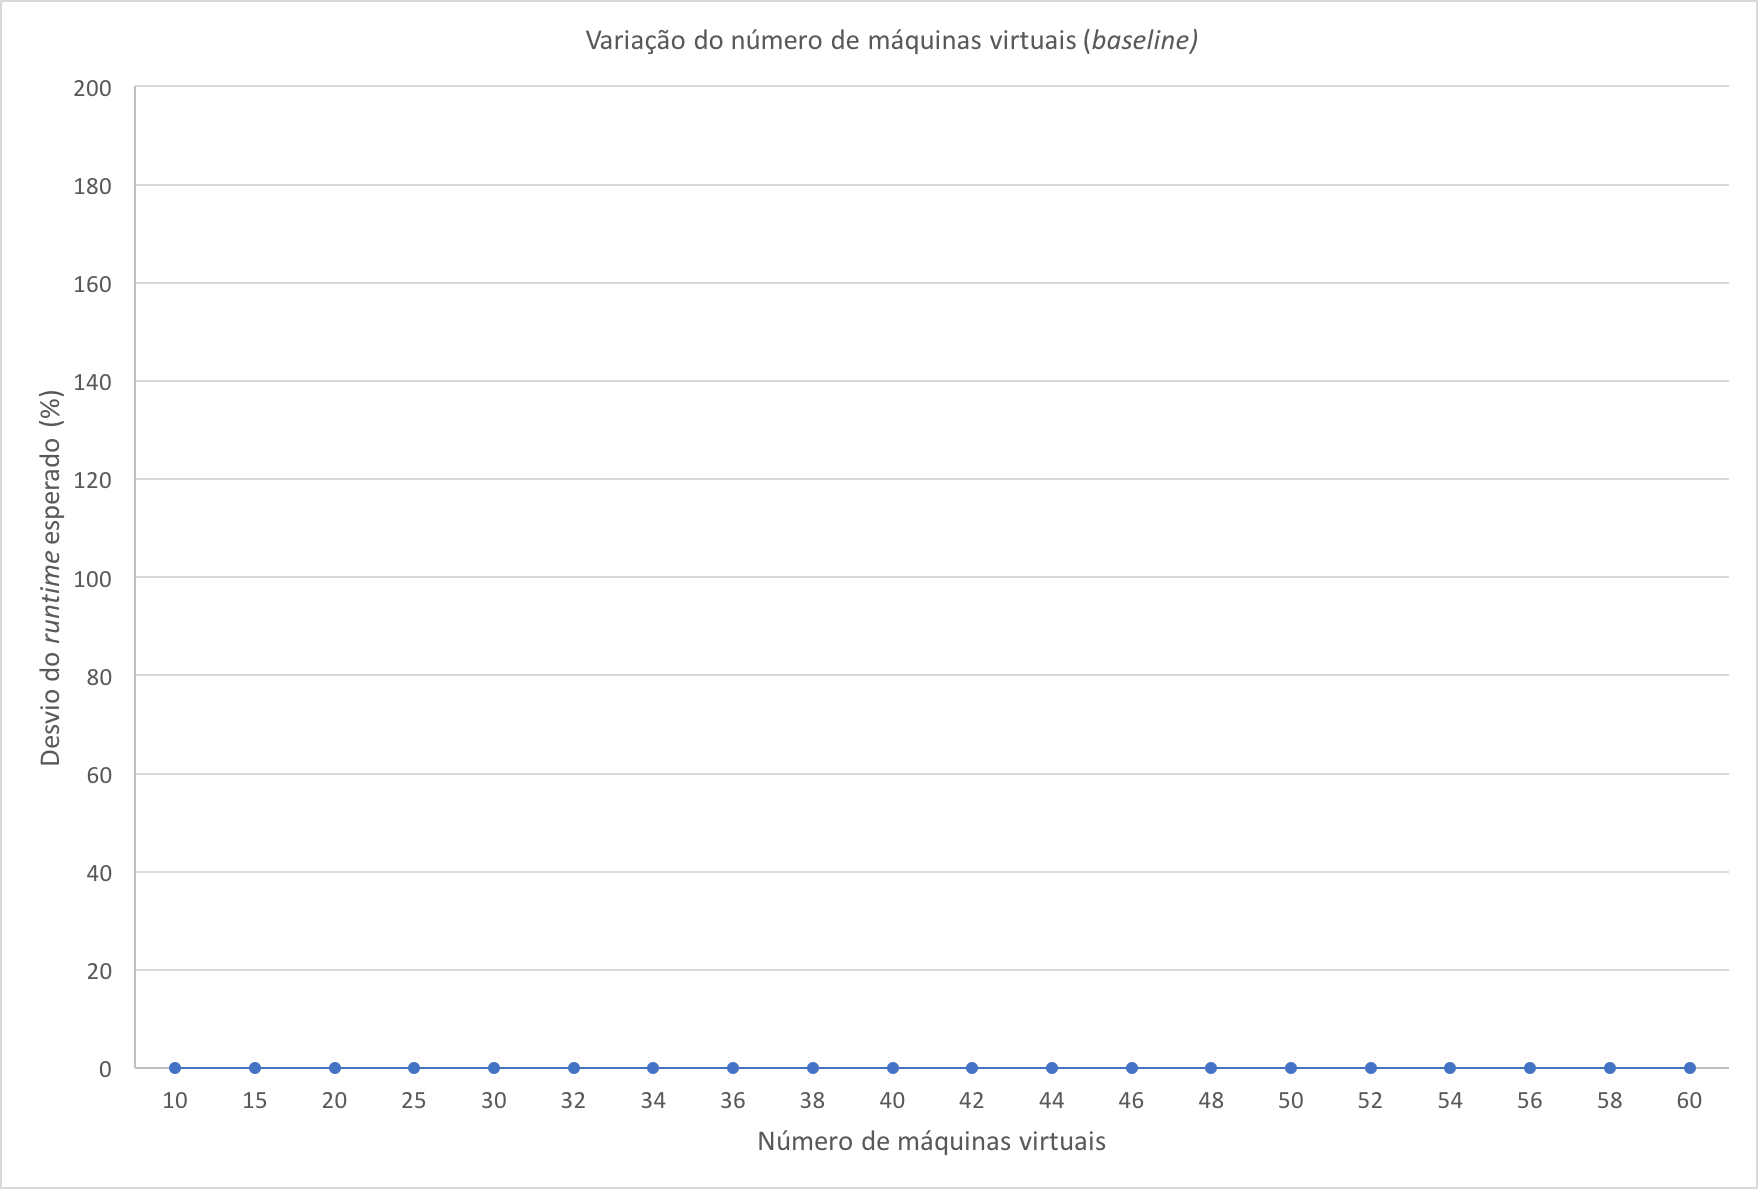
\includegraphics[scale=0.4]{figures/VMs/vms-nos-base.png}
			\caption{Máquinas Virtuais - Variação de inserções por minuto em modo \textit{baseline}}
			\label{fig:vms-ins-base}
		\end{figure}

		\discutir{faltam imagens e comentar}


\end{center}

